
\documentclass{standalone}

\usepackage{tikz} %Graphics
\usetikzlibrary{matrix}
\usepackage{amsmath}
\usetikzlibrary{shapes.geometric, arrows}


\tikzstyle{startstop} = [ draw=none, minimum width=1.5cm, minimum height=1cm, text centered]
\tikzstyle{process} = [rectangle, rounded corners, minimum width=1.0cm, minimum height=1.0cm, text centered, draw=black, fill=blue!30]
\tikzstyle{process_score} = [circle, minimum width=1.0cm, minimum height=1.0cm, text centered, draw=black, fill=blue!30]

\tikzstyle{arrow} = [thick,->,>=stealth]
\tikzstyle{arrow_back} = [thick,<-,>=stealth]

%\usetikzlibrary{...}
\begin{document}
	\begin{tikzpicture}[node distance=3.5cm]	
		\node (A) {
			\begin{tikzpicture}[every node/.style={anchor=base,
				text height=.8em,text depth=.2em,minimum size=7mm}]
			    \matrix[fill=blue!30, 		    
			            matrix of nodes, 
			            nodes={draw,minimum size=1cm}, 
			            nodes in empty cells,
			            column sep=-\pgflinewidth,
			            row sep=-\pgflinewidth]
			    (M)
			    {
					$a_{11}$   &   $...$   &   $max$  \\
					$...$   &   $...$   &   $...$  \\
					$a_{h1}$   &   $...$   &   $a_{hw}$ \\
				};
			\end{tikzpicture}
		};

		\node (af) [process, right of=A] {$MaxPool2d(A_i)$};
		\node (ao) [startstop, right of=af] {$a_o = max$};
		
		\draw [arrow] (A) -- (af);
		\draw [arrow] (af) -- (ao);
		
	\node (B) [below of = A] {
	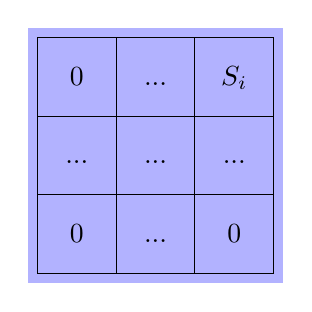
\begin{tikzpicture}[every node/.style={anchor=base,
		text height=.8em,text depth=.2em,minimum size=7mm}]
	\matrix[fill=blue!30, 		    
	matrix of nodes, 
	nodes={draw,minimum size=1cm}, 
	nodes in empty cells,
	column sep=-\pgflinewidth,
	row sep=-\pgflinewidth]
	(M)
	{
		$0$   &   $...$   &   $S_i$  \\
		$...$   &   $...$   &   $...$  \\
		$0$   &   $...$   &   $0$ \\
	};
	\end{tikzpicture}
};

	\node (sf1) [process, right of=B] {$S_o = S_i$};
	\node (so) [startstop, right of=sf1] {$S_o$};

	\draw [arrow_back] (B) -- (sf1);
	\draw [arrow] (so) -- (sf1);
		
	\end{tikzpicture}
\end{document}
